\section{Related Work}
We first inspect the traditional Softmax loss, an ordinary loss function used in classification-based models.
\begin{equation}
\label{equation01}
    L_{\text{Softmax}}=-\frac{1}{N}\sum\limits_{i=1}^{N}{\log }\frac{{{e}^{W_{{{y}_{i}}}^{T}{{x}_{i}}+{{b}_{{{y}_{i}}}}}}}{\sum\limits_{j=1}^{n}{{{e}^{W_{j}^{T}{{x}_{i}}+{{b}_{j}}}}}},
\end{equation}
where ${{y}_{i}}$ is the class to which the data ${{i}^{th}}$ belongs, $n$ is the number of labels, and $N$ is the number of samples. However, model using the Softmax loss function can only train with a fixed number of classes. It is obligatory to re-train the model if we want to add a new label. Siamese Network \cite{bromley1993signature} is one of the architectures that can work with new labels apart from the training set rather than re-train itself. Instead of classifying each input, we extract a feature vector, then compare it with the existing ones in the database to give decision. Thus, when adding a new label, we only need to add the vector of that label to the database.

\begin{figure}[htbp]
\label{figure01}
    \centering
    \centerline{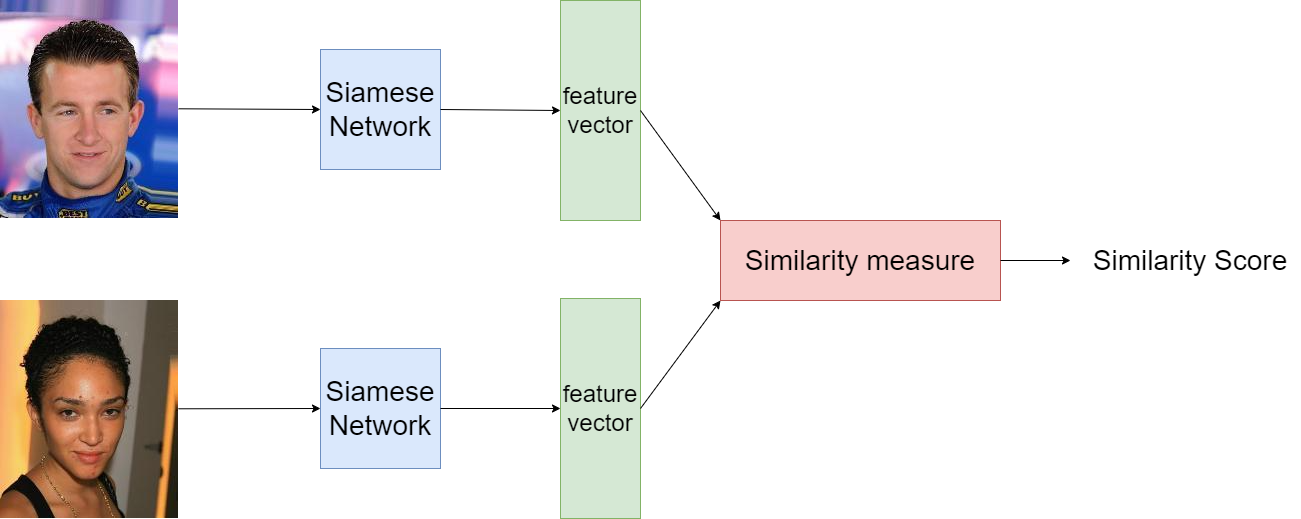
\includegraphics[width=\linewidth]{images/Siamese_Network.drawio.png}}
    \caption{Illustrate how the siamese model works. The image is taken from the CelebA \cite{liu2015faceattributes} dataset. The similarity measure could be cosine, euclidean, manhattan, etc.}
\end{figure}

Next, we transform the output logit \cite{pereyra2017regularizing} as $W_{j}^{T}{{x}_{i}}=\left\| {{W}_{j}} \right\|\left\| {{x}_{i}} \right\|\cos \left( {{\theta }_{ji}} \right)$, where ${{\theta }_{ji}}$ is the angle between the weight ${{W}_{j}}^{T}$ and the feature ${{x}_{i}}$. By $l_{2}$ normalization \cite{wang2017normface}, we set $\left\| {{W}_{j}} \right\|=\left\| {{x}_{i}} \right\|=1$, ${{b}_{j}}=0$, and having $s$ as a scale parameter, the original function (\ref{equation01}) becomes:
\begin{equation}
\label{equation02}
    L=-\frac{1}{N}\sum\limits_{i=1}^{N}{\log }\frac{{{e}^{s\cos {{\theta }_{{{y}_{i}}}}}}}{{{e}^{s\cos {{\theta }_{{{y}_{i}}}}}}+\sum\limits_{j=1,j\ne {{y}_{i}}}^{n}{{{e}^{s\cos {{\theta }_{ji}}}}}}.
\end{equation}
Established on the above function, some improved methods using margin value $m$ to increase performance.\\
\textbf{Liu et al.} \cite{liu2017sphereface}
\begin{equation}
\label{equation03}
    L_{SphereFace}=-\frac{1}{N}\sum\limits_{i=1}^{N}{\log }\frac{{{e}^{s\cos \left( m*{{\theta }_{{{y}_{i}}}} \right)}}}{{{e}^{s\cos \left( m*{{\theta }_{{{y}_{i}}}} \right)}}+\sum\limits_{j=1,j\ne {{y}_{i}}}^{n}{{{e}^{s\cos {{\theta }_{ji}}}}}},
\end{equation}
\textbf{Wang et al.} \cite{wang2018cosface}
\begin{equation}
\label{equation04}
    L_{CosFace}=-\frac{1}{N}\sum\limits_{i=1}^{N}{\log }\frac{{{e}^{s\left( \cos \left( {{\theta }_{{{y}_{i}}}} \right)-m \right)}}}{{{e}^{s\left( \cos \left( {{\theta }_{{{y}_{i}}}} \right)-m \right)}}+\sum\limits_{j=1,j\ne {{y}_{i}}}^{n}{{{e}^{s\cos {{\theta }_{ji}}}}}},
\end{equation}
\textbf{Deng et al.} \cite{deng2019arcface}
\begin{equation}
\label{equation05}
    L_{ArcFace}=-\frac{1}{N}\sum\limits_{i=1}^{N}{\log }\frac{{{e}^{s\left( \cos \left( {{\theta }_{{{y}_{i}}}}+m \right) \right)}}}{{{e}^{s\left( \cos \left( {{\theta }_{{{y}_{i}}}}+m \right) \right)}}+\sum\limits_{j=1,j\ne {{y}_{i}}}^{n}{{{e}^{s\cos {{\theta }_{ji}}}}}},
\end{equation}
and \textbf{Boutros et al.} \cite{boutros2022elasticface} $L_{ElasticFace}$, which its margin is a random value of the normal distribution.

Moreover, some other loss functions such as \textbf{Pairwise confusion loss} \cite{dubey2018pairwise}, \textbf{Triplet loss} \cite{schroff2015facenet}  use Siamese Networks to extract features and optimize the distance between the outputs.